\documentclass[runningheads]{llncs}
\usepackage{amssymb}
\setcounter{tocdepth}{3}
\usepackage{graphicx,epsfig}
\usepackage{algorithmic}
\usepackage{listings}
\usepackage{rotating}
\usepackage{subfigure}

%%%%

\usepackage{color}
\usepackage{alltt}
\usepackage{verbatim}
\usepackage{url}
\usepackage[latin1]{inputenc}
%\usepackage[spanish]{babel}



\usepackage{url}
\urldef{\mailsa}\path|rhgarcia@fidesol.org|
\urldef{\mailsb}\path|pgarcia@atc.ugr.es|
\urldef{\mailsc}\path|jmerelo@geneura.ugr.es|



\newcommand{\keywords}[1]{\par\addvspace\baselineskip
\noindent\keywordname\enspace\ignorespaces#1}

\lstset{
basicstyle=\ttfamily \scriptsize,
language=c++,
frame=single,
stringstyle=\ttfamily,
showstringspaces=false
}

\begin{document}
 %\pagestyle{empty} %ESTO QUITA LOS NUMEROS DE PAGINA
\mainmatter  % start of an individual contribution



% first the title is needed

\title{Emerging archetypes in massive artificial societies for literary purposes using genetic algorithms}


% a short form should be given in case it is too long for the running head
\titlerunning{Emerging archetypes in massive artificial societies for literary purposes}
%\author{R.H. Garc\'ia-Ortega\inst{1}, P. Garc\'ia-S\'anchez\inst{2} and J.J. Merelo\inst{2}}
\author{A.U. Thor\inst{1}}
%

%\authorrunning{R.H. Garc\'ia-Ortega et al.} 
% (FERGU): OJO! ES DOBLE CIEGO

% (feature abused for this document to repeat the title also on left hand pages)
% the affiliations are given next; don't give your e-mail address
% unless you accept that it will be published

%\institute{Fundaci\'on I+D del Software Libre, Granada, Spain \and Dept. of Computer Architecture and Technology, University of Granada, Spain 
%\mailsa, \mailsb, \mailsc\\}
\institute{Anonymous institute}


\maketitle


% -----------------------------------------------------------------------------
% ABSTRACT


\begin{abstract}

% Estructura actual del abstract:
% 1.- Hacer historias es muy complicado
% 2.- Entorno MADE: Cientos de personajes interactuando que permiten estudiar
%     los comportamientos
% 3.- Estudio de la parametrización y número de perfiles en el Entorno MADE 
%     para crear dos grupos de arquetipos: Control de natalidad y venganza
% 4.- Se usará un GA para encontrar la mejor solución (conjunto de parámetros)
% 5.- Se confirma la aparición de los arquetipos

The creation of fictional stories is a very complex task that usually
implies a creative process where the author has to combine characters,
conflicts and plots to create an engaging narrative. This work
presents a simulated environment with hundreds of characters that
allows the study of coherent and interesting literary archetypes (or
behaviours), plots and sub-plots. We will use this environment to
perform a study about the number of profiles (parameters that define
the personality of a character) needed to create two emergent groups
of archetypes: ``natality control'' and ``revenge''. A Genetic Algorithm
will be used to find the fittest number of profiles and parameter
configuration that enables the existence of the desired archetypes
(played by the characters without their explicit knowledge). The
results show that parametrizing this complex system is possible and
that these kind of archetypes can emerge in the given environment. 

\end{abstract}


% -----------------------------------------------------------------------------
% INTRODUCTION


\section{Introduction}
\noindent 

In videogames, NPCs (Non Player Characters)  are a type of characters that live in the game world to provide a more immersive experience. Modern RPGs (Role Playing Games), such as The Witcher\texttrademark~or Skyrim\texttrademark~count with hundreds of NPC characters. The effort to create a good interactive fiction script is directly proportional to the number of these characters. That is the reason this kind of agents usually counts with limited behaviours, such as wandering in the villages, selling groceries or guarding the cities. Also, they usually offer scripted conversations, for example, to buy and sell objects to the player. In other cases they interact with the player depending of the player's behaviour: for example, if the player steals something a city guard would attack him.  However, these characters do not interact among them, only with the player, and their activities are only guided with this purpose. In a world with such a number of characters, their collective interactions could improve the gaming experience, leading to a richer and more immersive world. For example, hungry inhabitants could become thieves, guards could pursuit the thieves, villagers could fell in love with others or different war alliances could emerge.

These facts have motivated us to develop a multi-agent system called MADE (Massive Artificial Drama Engine) to model a self-organized virtual world where their elements influences each other, following a cause-effect behaviours in a coherent manner. This system needs to be a suitable environment for the plot of a specific literary work, being also interesting for the player/spectator. A set of probabilities and states are associated to agents' actions, and these probabilities are optimized by means of an Evolutionary Algorithm (EA) to match with a specific literary archetype, defined by the fiction creator. The {\em archetypes} are behaviours and patterns universally accepted and present in the collective imaginary \cite{ArchetypesGarry05}, that allows empathize with the characters and immerse yourself in the story (for example, the well-known ``hero'' archetype).

In this work, several experiments have been carried out to answer the following questions: 

\begin{itemize}
 \item Is it possible to model a virtual environment inhabited by hundred of characters with interesting auto-generated behaviour based on literary archetypes?
 \item Could the personality of the agents be parametrized to obtain different behaviours? 
 \item How many profiles (groups of parameters that define a personality) are necessary to generate emergent quality sub-plots?
 \item Could a Genetic Algorithm be used to find the fittest parameter values that allow the creation of this kind of sub-plots?
\end{itemize}

In this paper we prove that EAs, together with a proper design of literary patterns, can be used to find the parameters that promote the generation of drama plots and sub-plots in a multi agent based environment.\\

The rest of the work is structured as follows: after the state of the art, the developed system is presented in Section \ref{sec:made}. Then, the experiments conduced with the EA are shown (Sections \ref{sec:experimentalsetup} and \ref{sec:results}). Finally, conclusions and future works are discussed.

% -----------------------------------------------------------------------------
% SEC SOA

\section{State of the art}
\label{sec:soa}

% (JJ): Por cierto, acabo de ver esto: \cite{StoryTecGobel2008}.
% (Rubén): TODO

Auto-generated interactive fiction research is mainly focused in methods to create the process of a story generation \cite{nairat2011character}. Story generation can be divided in two areas: interactive and non-interactive. In the first area, and according to \cite{ReviewArinbjarnar09}, an Interactive Drama is defined in a virtual world where the user has freedom to interact with the NPCs and objects in a dramatically interesting experience, different in each execution, and adapted to the interactions of the user.

The generation of interactive dramas can also be based in script
structure \cite{ArchitectureYoung04}, where each possibility in the
story must be previously defined, so there is a limited number of
possible plot combinations.

On the other side, in non-interactive plot generation systems the user does not take control as the protagonist. For example, in the system presented by Pizzi et al. \cite{pizzi2007interactive} the user can interact with the characters, changing their emotions, but making the user an spectator, rather than an actor.

As opposed to those concepts, MADE is focused in Artificial Non Interactive Drama, because its aim is the massive generation of plots for secondary characters, to provide a context for the writer and the player to perceive a virtual world as coherent, detailed and enriched. The story generation (that is, the narrative) is not addressed by MADE, but it has been studied in the systems presents in the survey by Arinbjarnar et al. in \cite{ReviewArinbjarnar09}.

% (JJ): Decir qué te hace suponer que esto va a ser una buena solución.
% (Rubén): TODO

Previous works define the plot as an emergence for the behaviour of the agents that follow a set of rules. In MADE, the agents' behaviour is product of its personality and the environment. That is, the agents does not follow the plot, but they generate the plot itself. 


Furthermore, the previous works generate plots in worlds with a limited number of characters. This restriction does not exist in MADE, where the number of characters to create is unlimited.



Following the ideas of the work of Epstein and Axtell
\cite{epstein1996growing} an environment based in {\em Sugarscape} has
been developed, with concepts such as food, metabolism and
vision. This environment uses the elements by Gershenson %nunca coma
                                %antes de verbo - JJ
\cite{gershenson2005general}: a virtual world, agents who born, grow,
interact, reproduce and dead; resources (food), mediators, and
relations of rivalry (friction) and cooperation (synergy). The actions
of these agents are parametrized according the work of Nairat
\cite{nairat2011character}, based in the use of genetic algorithms to
obtain a plot (solution) where two characters interact in a creative way.
 
%The current experiment allows the definition of behaviour patterns (or
%archetypes, and using a weighted fitness function to measure
%the presence of the desired archetypes. 



% -----------------------------------------------------------------------------
% SEC MADE

\section{The MADE Environment}
\label{sec:made}

The MADE environment is a virtual place where different agents play their artificial lives. Its functions are:

\begin{itemize}
\item \textbf{Create an initial set of agents:} MADE environment
  initializes a set of just born orphan agents, each with a profile
  sequentially assigned.
% (JJ): Sequentially de qu� secuencia? - JJ
% (Rubén): TODO
 These agents must compete or collaborate in order to survive.
\item \textbf{Place agents in the map:} the environment has a squared map, formed by cells that can be occupied by one (and only one) agent. The environment allows the agents to discover and interact with other agents in the neighbourhood.
\item \textbf{Start and control the time:} after the creation of the initial set of agents, the MADE environment starts the timer, day by day until a maximum date is reached.
\item \textbf{Execute each agent during a time unit (a day):} In each iteration the list of agents is randomly reordered, and after that following the new order, each agent perform an iteration of its life-cycle, and the dead agents are removed from the grid.
\item \textbf{Perform as an external agent that changes th environment:} In each iteration in the MADE environment, food rations are placed in random cells. An agent only can eat if it is over a cell with a ration, so agents could move the other forcibly.
\item \textbf{Offer services to the agents:} MADE environment allow the agents to check which closer cells have food, are occupied, who agents are in a near position or which positions can be occupied.
\item \textbf{Decide the profile of the agents:} MADE allows the existence of different agent profiles, as previously said. A {\em profile} is a set of characteristics which governs the agent's behaviour.
\end{itemize}

The MADE environment can be configured by using the following parameters (and its values by default): Number of agents initially placed (15), map square grid dimension (10), number of rations randomly placed in the grid each day (10) and duration in virtual days of the  execution of the environment (1000). Those parameters can affect directly to the behaviour of the agents.

% (JJ): Usas un estilo demasiado conciso. Di qu� hace cada uno de esos
% par�metros, c�mo se meten (fichero de configuraci�n o como sea), por
% qu� se eligen esos y no otros, y los valores por defecto que has
% usado. 

% (Rubén): por simplificar y reducir tamaño, pongo los valores por omisión


\subsection{MADE Agent}
A MADE Agent lives in a MADE Environment, occupies a cell in the grid, moves around looking for food or mate and interacts with other agents.

A very simple agent has been designed for this study: a virtual rat. We have modelled 4 states for it (be alive, be hungry, look for mate and be pregnant), 7 actions (move, eat, attack, defend, escape, find mate and have offspring) and parameters that define its characteristics and probabilities to perform actions depending on the state. It's important to remark that no ``feelings'' and no ``memory'' have been modelled in the MADE agent for this study.

Figure~\ref{fig:madeAgent} illustrates the nature of a MADE Agent.

\begin{figure}
\begin{center}
\includegraphics[scale=0.65]{img/MadeAgent.pdf}
\caption{Actions and states modelled in the MADE Agent.}
\label{fig:madeAgent}
\end{center}
\end{figure}

The life cycle of a MADE Agent illustrated in Figure~\ref{fig:lifecycle} represents on day in its life. Every decision made by the agent is based on its state and its characteristics (probabilities to perform different actions).

\begin{figure}
\begin{center}
\includegraphics[scale=0.32]{img/life_cycle.pdf}
\caption{MADE Agent's life cycle}
\label{fig:lifecycle}
\end{center}
\end{figure}

% (Rubén): TODO ¿citar todas las características de un agente made?
% Sólo si hay hueco, creo
% No se ve nada y no aporta mucho. No uses notaci�n del programa, sino
% del algoritmo. Y mejor que lo contaras como un algoritmo usando el
% entorno algorithmic que este gr�fico. - JJ

% (Rubén): TODO No se cómo mejorarlo...


The MADE Agent is created using 12 parameters, that define its base features and probabilities to make the decisions presented in the life-cycle of the Figure \ref{fig:lifecycle}. The execution of an agent is dynamic, and depends on the internal probabilities and states but also on the neighbourhood, and the map configuration. Even so, we can say that these initial parameters define in some way the possible situations where the agent could be involved.


\subsection{MADE Execution}

Every agent has a log or log that stores all the relevant events in its life in a simple format. Each line of the log indicates the day, the event in a short readable format and some extra information. Every agent's log in the MADE Environment is coherent with all others' logs. Many plots are being created, with a structured format that can be read by game engines or natural language processors, but, given the simplicity of the modelled agents, the stories could be seen by the reader as non-interesting. This log can be used for evaluation. In the next section we propose a method based on EA to let the author of a story promote different behaviours in the MADE agents that could be seen as literary archetypes (usually associated with human feelings and high level cognitive and memory abilities) that can be used to model NPCs in videogames (or be used in other creative areas). 

% -----------------------------------------------------------------------------
% SEC EXPERIMENTALSETUP

\section{Experimental setup}
\label{sec:experimentalsetup}

Thanks to the agents' logs, we can know every event (internal and external) of their lives, and evaluate their interest. In this work, we have implemented a method based in regular expressions with backreferences. The proposed technique puts annotations in every agent whose log matches a complex regular expression able to find emerging high level behaviours, not implemented in the life-cycle. 

In this proposal, the parameters used to define an agent, mentioned in Section~\ref{sec:made}, are mapped into a chromosome, and a Genetic Algorithm is used to evolve the solution. The fitness function is expressed in terms of:

\begin{itemize}
\item \textbf{Regular expressions applied to the log of each agent in the environment:} An agent is tagged when a regular expression matches its log.
\item \textbf{A numeric function over the number of tagged agents for each archetype:} the fitness of the solution is incremented with the returning value.
\end{itemize}

Different number of profiles (from 1 to 5) have been used to assign different parameters to different agents. If only one profile is used in a run, all the agents are created with the same parameters, evolved by the Genetic Algorithm. If more profiles are used, they are assigned to the agents in order of appearance in a loop. Our assumption is that some archetypes could emerge using one profile and other will need more (those that require two roles clearly differentiated). It's important to remark that the number of alleles of the chromosome are multiplied by the number of profiles, so the convergence of the solution could be affected by the number of profiles used.

For the experiments performed in this work, we have used the parameters shown in Table~\ref{fig:ga_parameters}. These values have been chosen empirically after several test runs. 

\begin{table}
\begin{center}
\caption{Parametrization of the Genetic Algorithm}
\label{fig:ga_parameters}
\begin{tabular}{p{3cm}p{7cm}}
\hline\noalign{\smallskip}
\noalign{\smallskip}
Parameter & Value \\
\hline
\noalign{\smallskip}
Codification & 12 alleles per profile\\
Fitness function & Average of 10 executions.\\
Natural selector & Original Rate: 0.9 \\
Crossover operator & Rate: 35\% \\
Mutation operator & Desired Rate: 12 \\
Stop condition & 100 executions\\
Generations & 30\\
Population size & 30 \\
\hline
\end{tabular}


\end{center}
\end{table}


% (JJ): Por qué has elegido estos experimentos y no otros? - JJ
% (Rubén): Done

For this work, two sample groups of archetypes (or scenes)  have been chosen: The first one is called ``natality control'' and its goal is to model a global archetype (population growth) and four individual memory based archetypes (\textit{downtrodden}, \textit{helpless}, \textit{warrior} and \textit{bad warrior}). The second scene is called ``revenge'' and its goal is to model an individual complex memory based behaviour between two characters (\textit{revenge}).


The Experiment 1, ``Natality control archetype'', aggregates different sample archetypes where many factors must be taken into account.  It tries to find what number of profiles and values are optimal to:
\begin{itemize}
\item Ensure that, after 1000 virtual days, the alive population will be the 60\% of the total population. This is called a \textit{global archetype}.
\item Emerge the \textit{downtrodden} archetype in the 22\% of the
  population. An agent will be considered as a \textit{downtrodden} or
  \textit{defender} if it has been attacked at least two times and has
  defended the position. 

\item Emerge the \textit{warrior} archetype the 22\% of the population. An agent will be considered as a \textit{warrior} if it has satisfactory attacked at least five times. 
\item Emerge the \textit{helpless} archetype the 22\% of the population. An agent will be considered as a \textit{helpless}  if it has been attacked at least ten times and hasn't defended the position.
\item Emerge the \textit{bad warrior} archetype the 22\% of the population. An agent will be considered as a \textit{bad warrior}  if it has unsatisfactory attacked at least ten times.
\end{itemize}
We have used the presented values to define this scene because, as our opinion, they model an interesting literary scene.

To model this group of archetypes we have defined the fitness function as follows:
If the exact percentage of agents are tagged with one archetype defined, 1 point is added to the fitness. The maximum is therefore, 5 points. However, all the archetypes use a normal distribution. For example, for the first archetype (``growing population''), the maximum value (1) is obtained when the 60\% percent of the population is alive, and the normal distribution begins in the 30\% and ends in the 90\%. For the rest of the archetypes, 1 point is added if the 22'5\% of the population is tagged with each one of the archetypes, and each normal distribution begins in the 8\% and ends in the 30\%.

% (Rubén) TODO: ¿Es interesante poner las expresiones regulares?

The experiment 2, ``Revenge archetype'', is performed to make more complex memory based behaviour emerge between two characters:  It tries to find what number of profiles and values are optimal to make \textit{revenge} archetype emerge in as many agents as possible after 1000 days.  An agent (a) will be considered as a \textit{avenger} if it has been attacked by other agent (b) and after that, in a moment in its life, it has satisfactory attacked the agent b, in revenge. The value of the days is set to 1000 because is a duration long enough to make the archetype emerge.

We have defined the fitness function of this experiment as follows:
For each agent, if the agent's log matches the archetype, it adds 1 point to the fitness. Therefore, the goal is to recreate an environment where most agents revenge.

The available source code of the MADE environment and the algorithms used in this experiment are publicly available in \url{http://ANONYMOUS} under a LGPL license. %AMOS, LA QUE TU QUIERAS, RUBEN (Fergu)

% (Rubén) TODO: ¿Es interesante poner las expresiones regulares?
% -----------------------------------------------------------------------------
% SEC RESULTS
\section{Results and discussion}
\label{sec:results}

Table~\ref{fig:exp1_30ex} shows the average of the best fitness and the average population fitness at the end of each execution for each configuration: number of profiles from 1 (P1) to 5 (P5) in the experiment 1 (``natality control'').
The evolution of the best fitness for each configuration is shown in Figure~\ref{fig:evo1}. We have performed a Kruskal-Wallis test for the best individuals fitness, obtaining differences among all the number of profiles (p-value $<<$0.05). As we suspected, it is clear that using one profile is not enough for emerge the desired archetype. However, the pairwise comparison using Wilcoxon does not find significant differences using more than 2 profiles. This can be explained because an agent could share more than one archetype at the same time.  A promising number of profiles could be 4, because their only lower outlier is not as distributed as the others. As can be seen in Figure \ref{fig:evo1} the evolution of the best fitness increases with all possible number of profiles, existing therefore an increase of the performance of the system.


\begin{table}
\begin{center}
\caption{Results for 30 executions of each configuration using 1 to 5 profiles in the experiment 1}
\label{fig:exp1_30ex}

\begin{tabular}{lllll}
\hline\noalign{\smallskip}
\parbox[t]{2cm}{Number of\\ profiles} 
& \parbox[t]{2cm}{Best fitness\\(average) *} 
& \parbox[t]{2cm}{Standard\\deviation}
& \parbox[t]{2cm}{Average\\fitness **}
& \parbox[t]{2cm}{Standard\\deviation}\\
\noalign{\smallskip}
\hline
\noalign{\smallskip}
1 & 0,765 & 0,037 & 0,761 & 0,038 \\
2 & 1,063 & 0,115 & 1,059 & 0,114 \\
3 & 1,093 & 0,063 & 1,091 & 0,062 \\
4 & 1,084 & 0,048 & 1,082 & 0,048 \\
5 & 1,045 & 0,110 & 1,041 & 0,108 \\
\hline
\end{tabular}
\\
\** Average of the best fitness at the end of each execution\\
% Es decir, coges el mejor fitness de cada ejecucion (tendras 30 por cada 
% numero de perfiles) y sacas la media
\*** Average population fitness  at the end of each execution \\
% Igual, pero la media del fitness medio en la última generación.
% Vamos, lo copias de la hoja de cálculo, lo que está en negrita.
\end{center}
\end{table}


The results of the second experiment (``revenge'') are shown in Table~\ref{fig:exp2_30ex}. It shows the average of the best fitness and the average population fitness at the end of each execution for each configurations. Boxplots of the best fitness obtained are shown in Figure \ref{fig:subfig2}. In this case, Krukal-Wallis and Wilcoxon pairwise comparison shows significant differences among all configuration (p-value $<<$ 0.05) except between P2 and P3 (p-value=0.3). Therefore, we can conclude that in this kind of global archetype only a profile must be used for obtaining the best results. This makes sense, because we are looking for one type of local archetypes ({\em avenger}), so adding extra profiles leads to different behaviours of the agents.


\begin{table}
\begin{center}
\caption{Results for 30 executions of each configuration using 1 to 5 profiles in the experiment 2}
\label{fig:exp2_30ex}
\begin{tabular}{lllll}
\hline\noalign{\smallskip}
\parbox[t]{2cm}{Number of\\ profiles} 
& \parbox[t]{2cm}{Best fitness\\(average) *} 
& \parbox[t]{2cm}{Standard\\deviation}
& \parbox[t]{2cm}{Average\\fitness **}
& \parbox[t]{2cm}{Standard\\deviation}\\
\noalign{\smallskip}
\hline
\noalign{\smallskip}
1 & 495,513 & 20,091 & 493,908 & 19,884 \\
2 & 471,206 & 24,550 & 469,361 & 24,015 \\
3 & 455,42 & 28,240 & 452,787 & 29,438 \\
4 & 431,926 & 31,682 & 428,206 & 31,238 \\
5 & 411,24 & 25,023 & 408,387 & 23,829 \\
\hline
\end{tabular}
\\
\** Average of the best fitness at the end of each execution\\
% Es decir, coges el mejor fitness de cada ejecucion (tendras 30 por cada 
% numero de perfiles) y sacas la media
\*** Average population fitness  at the end of each execution \\
% Igual, pero la media del fitness medio en la última generación.
% Vamos, lo copias de la hoja de cálculo, lo que está en negrita.
\end{center}
\end{table}

\begin{figure}[htb]
\centering

\subfigure[Experiment 1]{
   \includegraphics[width=13.5pc] {img/exp1_v2.pdf}
   \label{fig:subfig1}
 }
\subfigure[Experiment 2]{
   \includegraphics[width=13.5pc] {img/exp2_v2.pdf}
   \label{fig:subfig2}
 }
\caption{Average fitness of the 30 best individuals for each configuration.}

\label{fig:graph}
\end{figure}

\begin{figure}[htb]
\centering

\subfigure[Experiment 1]{
   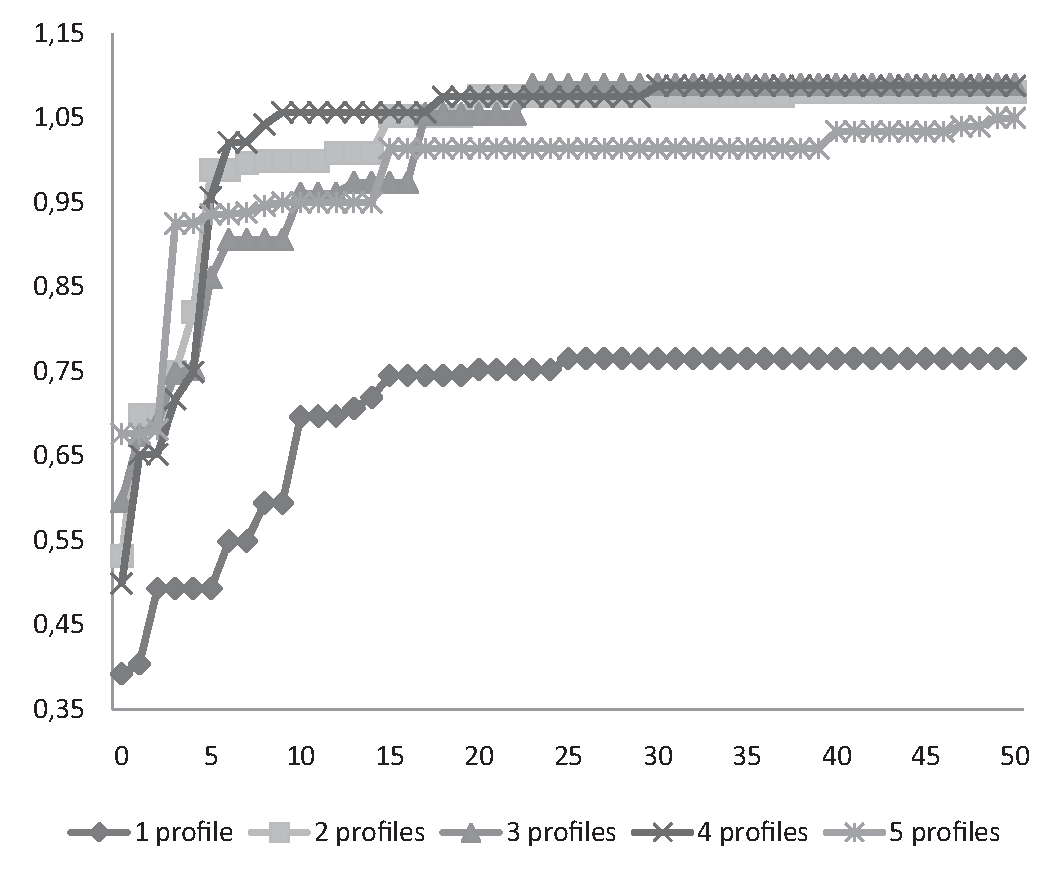
\includegraphics[width=13.5pc] {img/graph1_v2.pdf}
   \label{fig:evo1}
 }
\subfigure[Experiment 2]{
   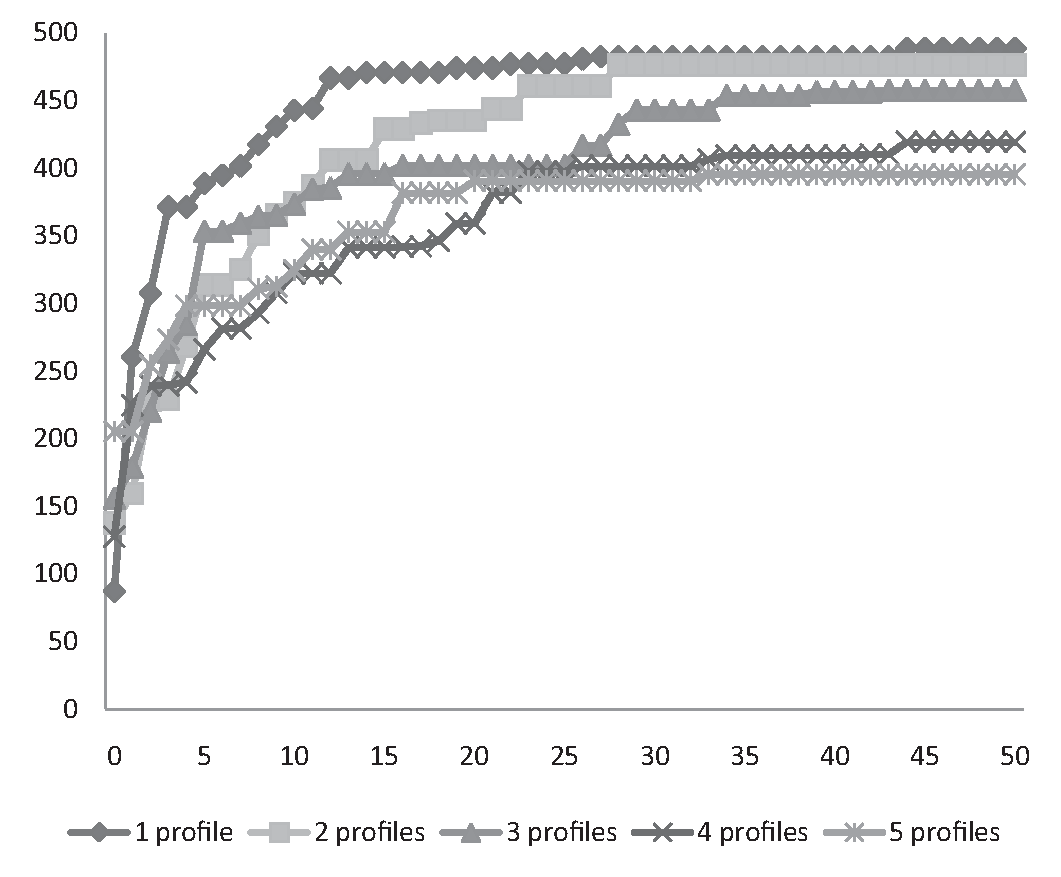
\includegraphics[width=13.5pc] {img/graph2_v2.pdf}
   \label{fig:evo2}
 }
\caption{Example of the evolution of the best individual for the 5 profiles for each configuration.}

\label{fig:boxplots}
\end{figure}

\clearpage


% -----------------------------------------------------------------------------
% SEC CONCLUSIONS

\section{Conclusions}
\label{sec:conclusion}

This work presents the MADE environment, a self-organized multi-agent system to model complex societies. This system can be used to study emergent behaviours for literary purposes, for example, to extract interesting plots for NPCs in videogames. In this work we have used the MADE environment to establish the number of profiles (sets of personality parameters) necessary to emerge two different global archetypes: ``natality control'' and ``revenge''. We have used a Genetic Algorithm to optimize the parameters of these profiles using as a fitness a function that model the two desired global archetypes. Results show that in the first archetype the number of profiles must be at least two, because it is necessary that different behaviours (local archetypes) emerge. On the contrary, on the second experiment, using only one profile is the best configuration, because the purpose was to emerge only one archetype ({\em avenger}). If the number of profiles is increased worse results are obtained.

In future works, more complex agents will be used, with different rules to be modelled. For example, we plan to model more human behaviours such as love or envy, to generate interesting plots such as wars, weddings, or family crimes. Different fitnesses will be used, for example, taking into account human opinions to establish the interestingness of a generated plot. Also, this system will be tested into an existent and well-known game, such as Skyrim\texttrademark, whose AI engine is publicly available for players and researchers.

% -----------------------------------------------------------------------------
% SEC ACKNOWLEGGEMENTS

\section*{Acknowledgements}
%This work has been supported in part by FPU research grant AP2009-2942 and projects EvOrq (TIC-3903), CANUBE (CEI2013-P-14) and ANYSELF (TIN2011-28627-C04-02).

\bibliographystyle{splncs}
\bibliography{made}

\end{document}

